\section{Autopilots --- Two Loops, Root-Locus Design}

Between the guidance command and the fins sits the autopilot. Two identical autopilots are used, one for pitch and one for yaw, each built as a nested pair of loops and designed by root locus (\texttt{ProjRLocus.m}). The three loops are:

\begin{enumerate}
    \item \textbf{Inner (rate gyro):} feeds back the body rate $q$ (or $r$) and damps the short-period. This is what turns the lightly damped airframe of Section~\ref{sec:dyn} into a well-behaved plant, raising the damping from $\xi\approx 0.08$ to $\approx 1$.
    \item \textbf{Outer attitude:} a proportional term plus an integrator tracking $q\rightarrow\theta$, with the gain chosen on the root locus where the dominant damping is $\zeta\approx 0.5$. It is used in cruise, driven by the altitude controller.
    \item \textbf{Outer acceleration:} an integrator $-1/s$ tracking the lateral acceleration, with the highest gain that keeps the dominant damping $\zeta_{dom}\geq 0.6$. The gain is bounded by the non-minimum-phase zero of the acceleration transfer function. It is used in the terminal phase, driven by proportional navigation.
\end{enumerate}

The gains are selected on the root locus of each loop, sweeping the design across the full flight condition (Section~\ref{sec:sched}).

\begin{figure}[H]
\centering
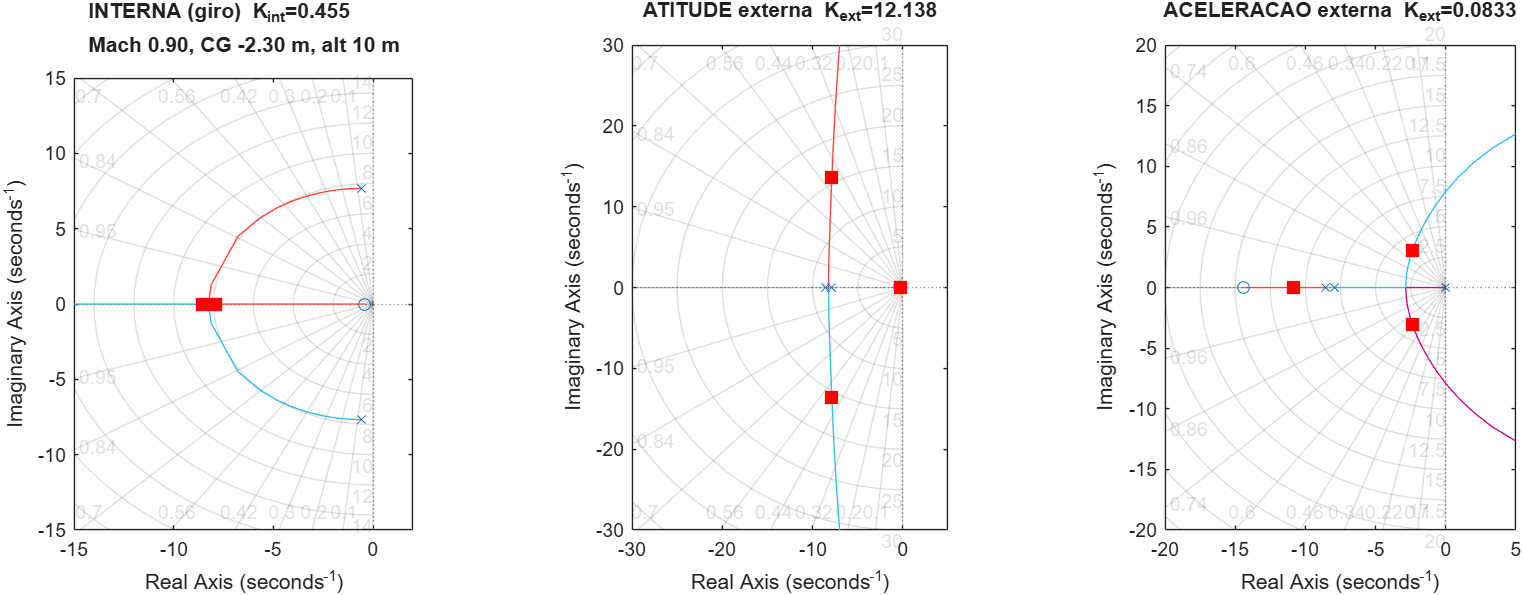
\includegraphics[width=0.92\textwidth]{figures/root_locus.png}
\caption{Root locus of the three loops; the square marks the selected gain.}
\end{figure}

\subsection{Autopilot Model in Simulink}

The autopilot is implemented as the \texttt{Autopiloto} subsystem of \texttt{GuiamentoControle.slx}. Figure~\ref{fig:ap_harness} shows the test harness used to design and verify it in isolation: pulse generators inject attitude/acceleration commands, the autopilot drives the fin deflections $\delta_y$ and $\delta_z$, and the 6DOF block returns the airframe response, which is fed back to the autopilot.

\begin{figure}[H]
\centering
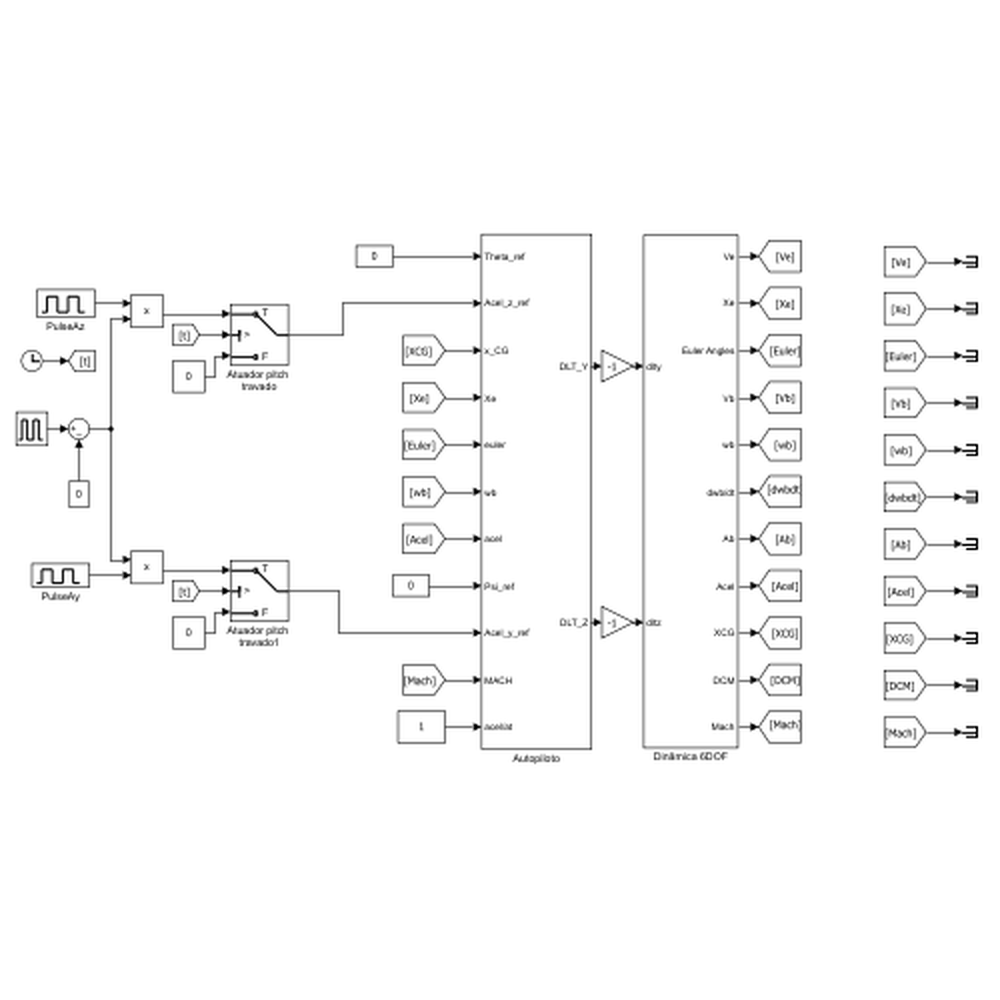
\includegraphics[width=0.86\textwidth]{figures/simulink_autopilot_harness.png}
\caption{Simulink test harness for the autopilot: command generators (left) drive the \texttt{Autopiloto} subsystem, which commands the \texttt{Din\^amica 6DOF} block; the response is fed back. The \emph{actuator-lock} switches (\texttt{Atuador pitch travado}) force $\delta=0$ during the boost.}
\label{fig:ap_harness}
\end{figure}

Internally, the \texttt{Autopiloto} subsystem is organized in clearly separated sections. Each channel (pitch/yaw) contains an attitude tracker and an acceleration tracker in parallel, and a switch selects which one is active according to the flight mode. Figure~\ref{fig:ap_blocks} shows the architecture of a single channel and Table~\ref{tab:ap_blocks} describes each section.

\begin{figure}[H]
\centering
\begin{tikzpicture}[
  >=Latex, node distance=7mm and 10mm,
  block/.style={draw, rounded corners, minimum height=8.5mm, minimum width=15mm, align=center, font=\scriptsize},
  sum/.style={draw, circle, inner sep=0pt, minimum size=4.5mm, font=\scriptsize},
  every node/.style={font=\scriptsize}
]
  \node (ref)  {$\theta_{ref}/A_{ref}$};
  \node[sum, right=8mm of ref] (s1) {};
  \node[block, right=of s1] (kext) {$K_{ext}$\\(lookup)};
  \node[sum, right=8mm of kext] (s2) {};
  \node[block, right=of s2] (act) {actuator\\+ sign $-1$};
  \node[block, right=of act] (sat) {sat\\$\pm 20^\circ$};
  \node[block, right=of sat] (air) {airframe\\$\delta\!\to\!q,\theta,A_z$};
  \node[right=9mm of air] (out) {$\theta/A_z$};

  \draw[->] (ref) -- (s1);
  \draw[->] (s1) -- (kext);
  \draw[->] (kext) -- (s2);
  \draw[->] (s2) -- (act);
  \draw[->] (act) -- (sat);
  \draw[->] (sat) -- (air);
  \draw[->] (air) -- (out);

  % inner rate-gyro loop
  \node[block, below=9mm of s2] (kint) {$K_{int}$ (lookup)\\ $\times\,q$};
  \draw[->] (air.south) |- (kint.east);
  \draw[->] (kint) -- (s2) node[midway,left]{$-$};

  % outer feedback
  \coordinate[below=17mm of air] (fb);
  \draw[->] (out) |- (fb) -| (s1) node[pos=0.98,left]{$-$};
\end{tikzpicture}
\caption{Architecture of one autopilot channel: outer loop (gain-scheduled $K_{ext}$, attitude or acceleration), inner rate-gyro loop (gain-scheduled $K_{int}$ on $q$), actuator with sign inversion and $\pm 20^\circ$ saturation, and the airframe transfer functions.}
\label{fig:ap_blocks}
\end{figure}

\begin{table}[H]
\centering
\caption{Sections of the \texttt{Autopiloto} subsystem and their function.}
\label{tab:ap_blocks}
\begin{tabular}{p{0.27\textwidth}p{0.65\textwidth}}
\toprule
Section / block & Function \\
\midrule
Demux of inputs & Splits the incoming vectors into the signals each loop needs: attitude $\theta,\psi$ from \texttt{euler}, rates $q,r$ from \texttt{wb}, accelerations $A_z,A_y$ from \texttt{acel}, and the scheduling variables (altitude, Mach, $x_{CG}$). \\
Actuator-lock switch & During the first $T_{Trav}$ (boost) it forces $\delta=0$: the missile is still accelerating and the fins are held. After $T_{Trav}$ the command passes through. \\
Attitude tracker & Outer loop for cruise. Computes the attitude error $\theta_{ref}-\theta$, applies the gain-scheduled external gain, and subtracts the inner rate-gyro signal. Used with the sea-skim altitude controller. \\
Acceleration tracker & Outer loop for homing. Same inner structure, but with an integrator $1/s$ on the acceleration error so the steady-state error is zero. Used with proportional navigation. \\
Mode selector (switch) & Selects the active tracker (attitude vs.\ acceleration) from the \texttt{At/Acel} flag set by Guidance \& Control. \\
Gain-scheduled lookups & Each loop reads its gain from a 3D table $T(x_{CG},\text{alt},\text{Mach})$ interpolated in real time (Section~\ref{sec:sched}). \\
Actuator + sign inversion & The commanded deflection passes through the actuator with a $-1$ gain, correcting the sign convention of the $\delta\rightarrow q$ transfer function (Section~\ref{sec:sign}). \\
Saturation $\pm 20^\circ$ & Hard mechanical limit of the fin; the autopilot output can never exceed it, independently of the command. \\
\bottomrule
\end{tabular}
\end{table}

\subsection{Gain Scheduling}
\label{sec:sched}

A single fixed set of gains cannot fly the whole mission, because the plant changes with the flight condition. The gains vary strongly with \emph{Mach} (through the dynamic pressure $\bar q$, which scales all aerodynamic forces) and with the \emph{CG position} (through the static margin, which changes as propellant burns), and only weakly with \emph{altitude}. The design therefore sweeps six CG points (the five burn phases), two altitudes and three Mach numbers, and stores the resulting gains in three-dimensional tables $T_{xxx}(x_{CG},\text{alt},\text{Mach})$, saved to \texttt{autopiloto.mat}.

At run time, each autopilot loop reads its gain by interpolating (\texttt{interpn}) its table at the instantaneous flight condition. The scheduling grid uses $\text{Mach}=[0.6~~0.75~~0.9]$ and $\text{alt}=[10~~100]~\text{m}$. During the initial low-speed transient (below Mach $0.6$) the tables extrapolate, which is visible as a short transient in the flight time series but does not affect the cruise or terminal behavior.

\begin{figure}[H]
\centering
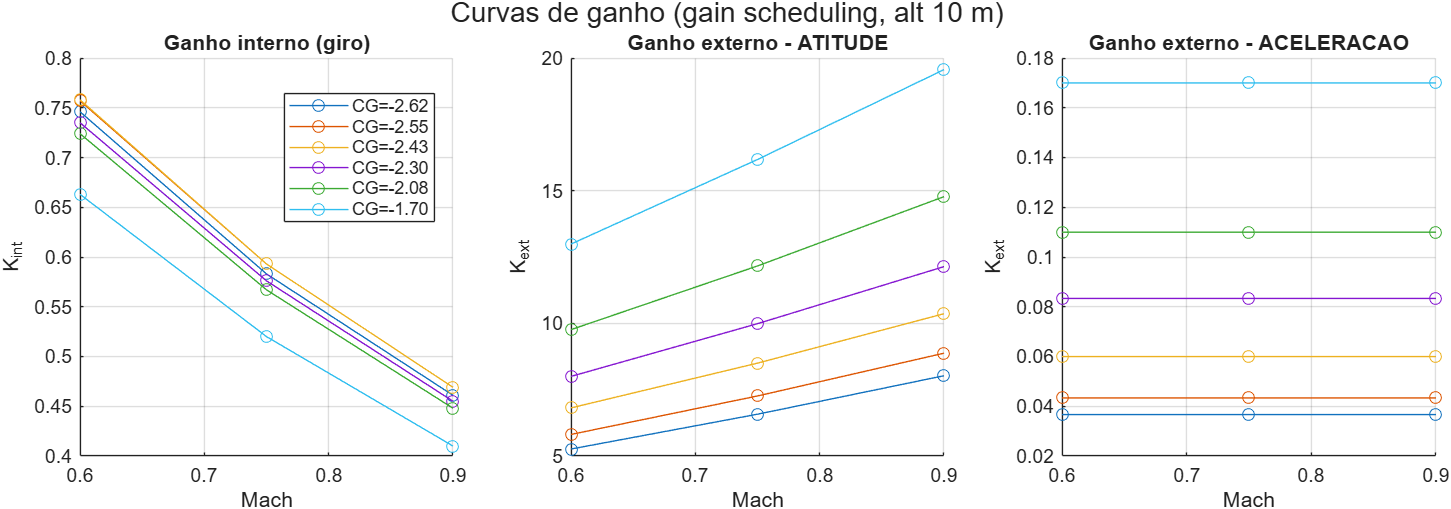
\includegraphics[width=0.9\textwidth]{figures/gain_schedule.png}
\caption{Gain schedule: internal and external gains versus Mach for each CG phase.}
\end{figure}

\subsection{Sign-Convention Correction}
\label{sec:sign}

This missile's $\delta\rightarrow q$ transfer function has \emph{negative} gain, the opposite convention to the anti-drone reference model the project started from. If nothing is done, the nominally negative feedback becomes positive: the loop destabilizes and the executed motion comes out inverted with respect to the command. This is not a tuning issue but a sign issue, so it must be fixed structurally.

Two coordinated corrections restore negative feedback and keep the design and the simulation consistent. In the gain design, the actuator enters the loop with a negated numerator ($\texttt{num\_at}=-\texttt{AT.num}$). In the simulation model, a $\text{Gain}=-1$ is placed on each autopilot deflection output (pitch and yaw); this same inversion also reconciles the DATCOM aerodynamic sign convention with the Simulink coordinate system. All four sign combinations (actuator $\pm$, gains $\pm$) were tested, and only the pair ``actuator negated with positive gains'' is stable, which is the one adopted.

\subsection{Performance --- Step Responses and Command Tracking}

The closed-loop autopilot is verified against the bandwidth requirement with attitude, acceleration and $5g$ steps, and then confirmed inside the full 6DOF simulation.

\begin{itemize}
    \item \textbf{Attitude step:} DC gain $=1.00$, $\approx 8\%$ overshoot, bandwidth $2.6$--$3.6~\text{Hz}$. The slow tail comes from the incidence zero.
    \item \textbf{Acceleration step:} DC gain $=1.00$, an initial dip caused by the non-minimum-phase zero, $\approx 8$--$10\%$ overshoot, bandwidth $0.7$--$1.3~\text{Hz}$.
\end{itemize}

A DC gain of $1.00$ means the output settles exactly on the command --- the autopilot follows what it is told. Both channels clear the $0.5~\text{Hz}$ requirement.

\begin{figure}[H]
\centering
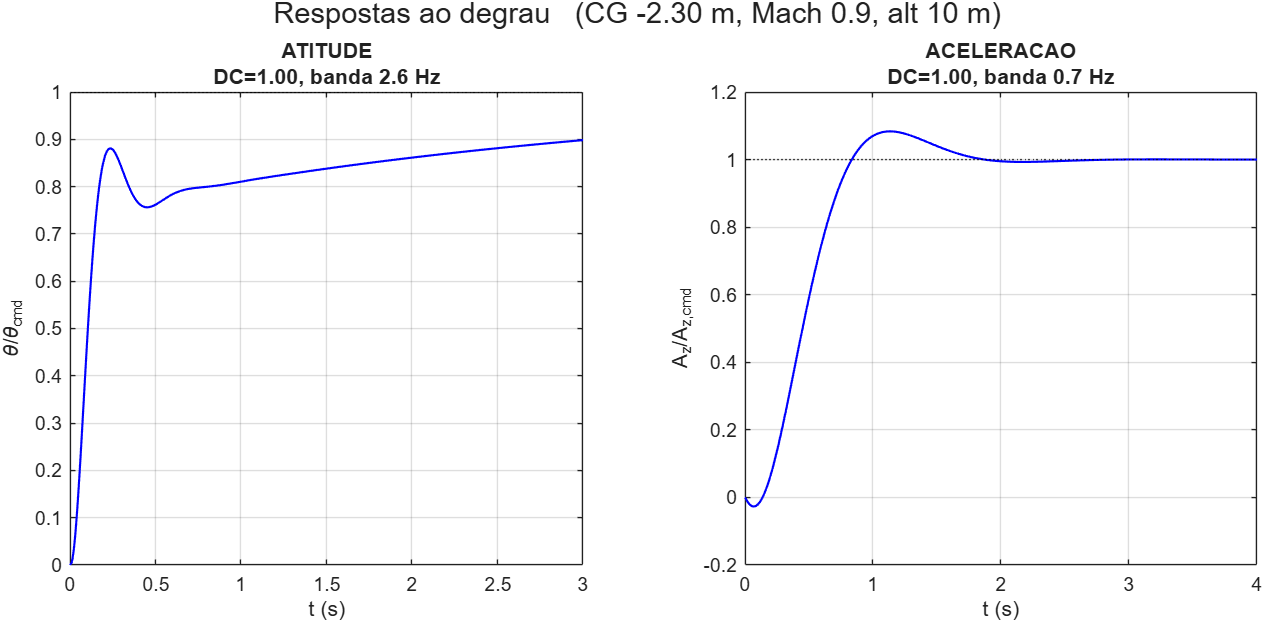
\includegraphics[width=0.88\textwidth]{figures/step_autopilot.png}
\caption{Attitude and acceleration step responses.}
\end{figure}

For the sizing $5g$ command, the simulated response reaches $5g$ faster than the $0.5~\text{Hz}$ bandwidth requirement (it overshoots to $\approx 5.48g$ and settles at $5g$), so the same design satisfies both the maneuver and the bandwidth requirements at once.

\begin{figure}[H]
\centering
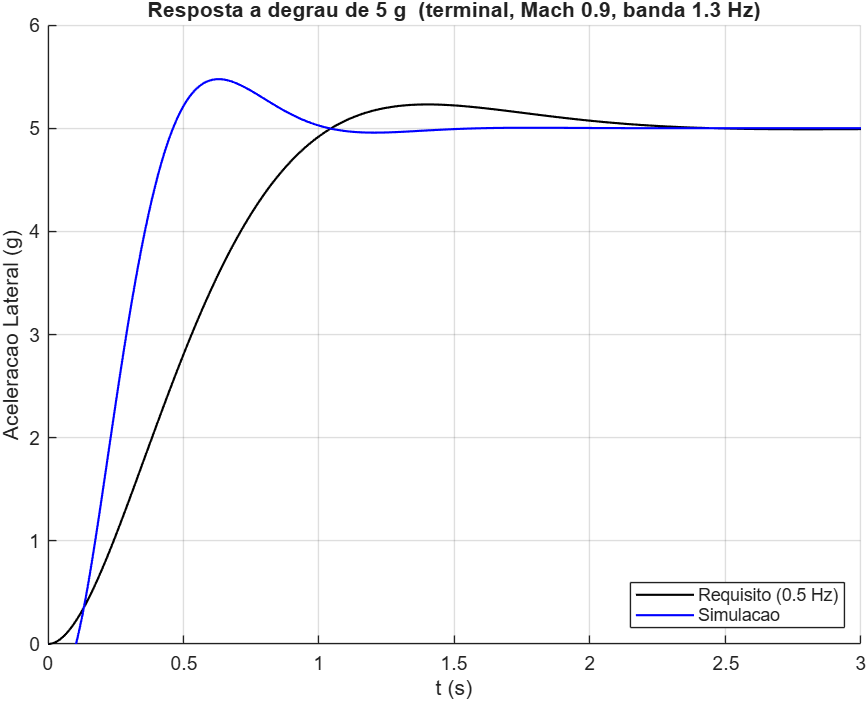
\includegraphics[width=0.78\textwidth]{figures/step_5g.png}
\caption{$5g$ step response against the bandwidth requirement.}
\end{figure}

Finally, in the complete 6DOF simulation the commanded and executed responses ($\theta$, $\psi$, $A_y$, $A_z$) practically coincide (Figure~\ref{fig:cmd_exec}), confirming that the scheduled autopilot tracks the guidance command across the whole flight, not only at the isolated design points.

\begin{figure}[H]
\centering
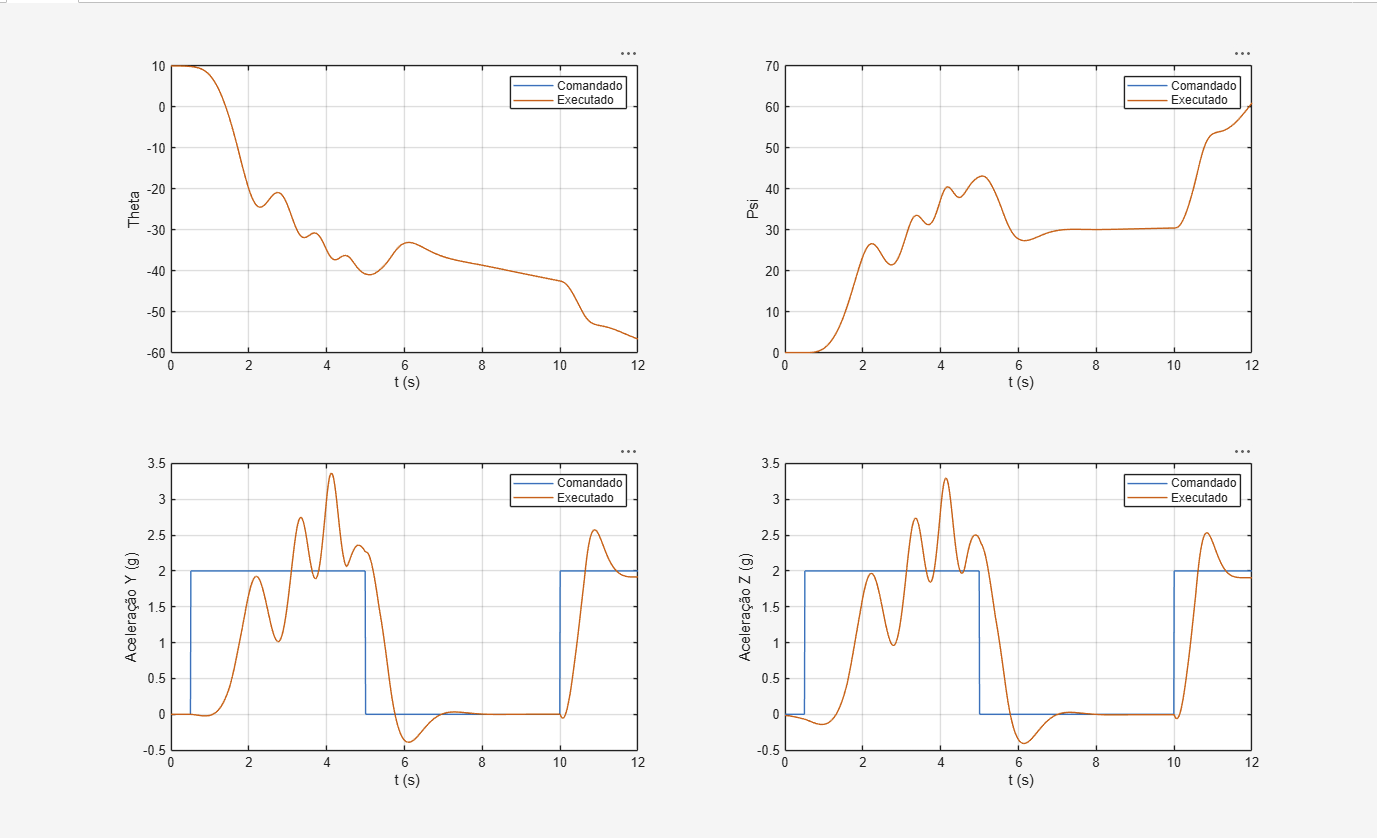
\includegraphics[width=0.86\textwidth]{figures/command_vs_executed.png}
\caption{Full 6DOF: commanded versus executed responses ($\theta$, $\psi$, $A_y$, $A_z$); the curves are nearly indistinguishable.}
\label{fig:cmd_exec}
\end{figure}
